\documentclass[main.tex]{subfiles}
\begin{document}
	
	\chapter{Perception}
		\chapterauthor{Jan-Frederik Stock, Evan Kapitzke,\\Leonidas Paniago De Oliveira Neto}
		
		\section{General}
		The main changes and improvements upon the status presented at milestone 1 are the following: Perception now runs inside an actionserver, in contrast to 				plain robosherlock. Additionally, Caffe is now used for feature extraction, and KNN is used for the classification of detected objects. Also, image data of 		available objects was recorded, which was then used for classification purposes.
		
		\section{Actionserver and process manager}
			\subsection{Interfaces}
			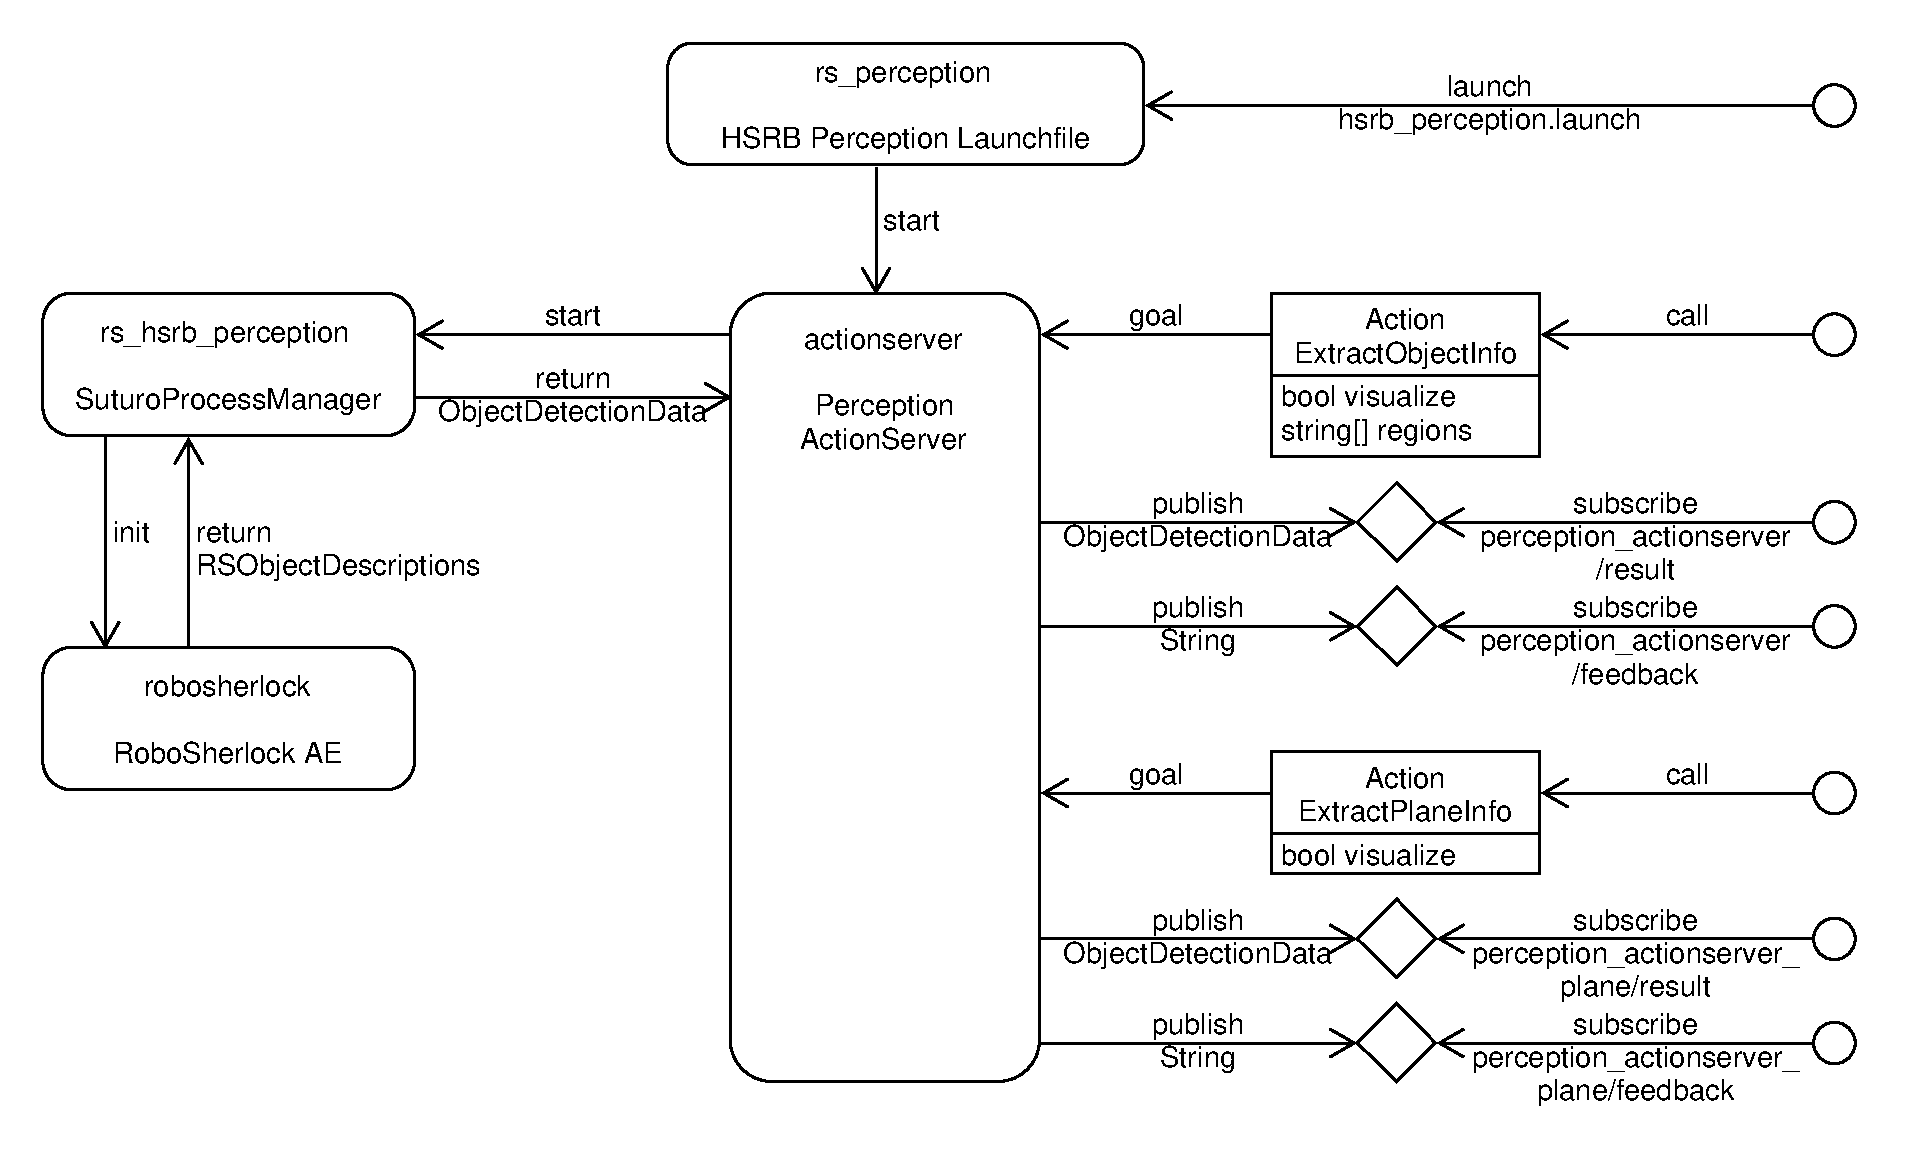
\includegraphics[width=\textwidth]{../architecture/perception_architecture/perception.pdf}
			
			\subsection{Packages}
			\subsubsection{Launch}
			In order to start the perception action servers you have to call:\\
			"roslaunch rs\_perception hsrb\_perception.launch".

			\subsubsection{actionserver}
			Implements the "ExtractObjectInfo" and "ExtractPlaneInfo" action servers and the corresponding action clients.
			Internally the "SuturoProcessManager" from "rs\_hsrb\_perception" is used to communicate with RoboSherlock.
			The action server invokes "SuturoProcessManager::run()" with the given parameters. 
			The executable "perception\_server" starts both action servers.
			Set "\_region:=\textbf{region\_name}" as parameter in "ExtractObjectInfo" to enable the RegionFilter.

			\subsubsection{rs\_perception}
			Includes launch-, configuration- and analysis descriptor files.\\
			To convert published URDFs to YAML run: "region\_filter\_setup.py" (originally from Suturo1819).\\
			Generated YAML map descriptors must be placed in the "config" folder.

			\subsubsection{rs\_hsrb\_perception (forked from suturo1819)}
			Implements a RoboSherlock process manager "SuturoProcessManager".
			The manager gets called from the "actionserver" and executes the selected pipeline once.
			
			In order to perceive objects that are placed on the ground, the SuturoRegionFilter gets reconfigured
			to disable the region filtering. Set the region parameter to \{ "robocup\_default" \} to enable this feature.

			The "RegionAnnotator" annotates the source region of perceived objects. Those regions are used
			to decide whether or not an object should be published, if the "regions" parameter is set.

			\subsection{Changelog}
			\begin{itemize}
			\item Changed pipeline descriptor and created new analysis engine descriptor for planes
			\item The actionserver package got created:
				\begin{itemize}
				\item ExtractObjectInfoServer - Instantiates a SuturoProcessManager with the "hsrb\_1ms" pipeline descriptor
				\item ExtractObjectInfoClient - Action client to test the ExtractObjectInfoServer
				\item ExtractPlaneInfoServer - Instantiates a SuturoProcessManager with the "hsrb\_planes" pipeline descriptor
				\item ExtractPlaneInfoClient - Action client to test the ExtractPlaneInfoServer
				\item perception\_server - Main executable, which initializes both action servers
				\end{itemize}
			\item Updated to the newest RoboSherlock version
			\item Fixed visualisation in the "SuturoProcessManager"
			\item Added SuturoRegionFilter:
				\begin{itemize}
				\item Based on RoboSherlock RegionFilter
				\item The RegionFilter is used to extract only points in a specific region. Those regions are defined in "suturo\_semantic\_map.yaml"
				\item Implemented "reconfigure()" to disable it without restarting the pipeline
				\end{itemize}
			\item Changed "RegionAnnotator" to work with "SemanticMapObject" instead of custom "Region" data type
			\item Fixed crash after loading an earlier annotated plane (caused by PlaneAnnotator)
			\end{itemize}

		\section{Classification}
		    \subsection{Feature Extraction}
		    In order to gain features on which to train classifiers, Caffe\footnote{\url{https://caffe.berkeleyvision.org/}}, in combination with the robosherlock 				package rs\_addons\footnote{\url{https://github.com/bbferka/rs_addons}} is used. rs\_addons was forked, off of another fork\footnote{\url{https://					github.com/Vanessa-rin/rs_addons}} to be able to make changes to the source code\footnote{\url{https://github.com/Jastock/rs_addons/tree/								rs_classifier_makeover}}.\\
		    
		    rs\_addons provides a program called "featureExtractor". It needs a split file, which specifies the classes your classifier will later output, as well 				as an output folder and the caffemodel to use as inputs. To make this process easier, shell scripts to generate a split file and a classlist from 					directory names can be found in \url{https://github.com/SUTURO/suturo_perception/tree/master/featureExtraction/tools}. Training images have to be 					provided as well, which have to be placed in the "object\_data" folder in the rs\_resources\footnote{\url{https://github.com/RoboSherlock/							rs_resources}} package. More information on how the training images can be recorded will be provided in the "Recording of images" section.\\
		    
		     Running this program will provide a file containing a matrix with features for every class specified in the split file. It also provides a file with a 			mapping from the classnames to the numbers used in the feature matrix to represent the classes. These files can now be used to train classifiers. For 				exact information on how to do feature extraction using this method, refer to \url{https://github.com/SUTURO/suturo_perception/blob/master/							featureExtraction/featureExtraction.md}. 
			
			\subsection{Classifiers}
			The newly generated files from the previous section can then be used in the annotators for classification provided by rs\_addons. Until now, the KNN-					Annotator was used for classification. The SVM-Annotator and the RF-Annotator were tested to make sure they work, but to use them effectively, their 					settings have to be tweaked.\\
			
			To find out which of these methods for classification works best for this specific problem, they have to be objectively compared. Up to this point, 					there is no effective way of doing this. The implementation of such a way is a goal for the next milestone. The idea is to implement a tool that 						can be used to label the objects in an example scene. A different tool can then run classification algorithms on these labeled scenes and calculate 					evaluation criteria, such as accuracy, recall, precision and the f-score. The tool should also be able to evaluate the speed of the algorithms. On the 				basis of these criteria, the algorithms can be objectively compared and the best one for the problem at hand can be selected.
			
			\subsection{KNN Confidence}
			In the official version of rs\_addons the confidence for a prediction is calculated by only looking at the distance of the first neighbor to the new 					sample. This is not a sufficient representation and it does not show difference when choosing different K's. To fix this, a new version of the 						confidence was implemented by dividing the number of neighbors belonging to the result class by the total number of neighbors, in other words the K.
			The new version can be found in \url{https://github.com/Jastock/rs_addons/blob/rs_classifier_makeover/src/classifiers/RSKNN.cpp}, in the 								"calculateConfidence" function.  
			
			\subsection{Saving the classification results}
			To be able to compare and visualize the classification results, the classificationEvaluation package was implemented. It provides an actionclient, that 			sends action goals to the perception actionserver and receives the results. These results can be represented in a markdown table or plotted in a 						scatterplot. By leaving the "rsClassificationEvalutator" node running and stopping the actionserver to alter the configuration, different K's can be 					tested and saved in case of using KNN. The package can be found here: . 
		
		
		\section{Recording of images}  
		Image capture is the first step to classification with the main goal in creating a big dataset
		for the Robocup containing objects from several supermarkets.
		The process is composed of starting the camera driver,
		finding the right plane and taking pictures while turning the object.
		First we need to install the driver for the camera and for this we use OpenNi 2
		then OpenNi 2 work as a driver for the camera and as interface to ros.
		For easy use we have a shell script that will download all needed dependencies
		and make changes on the package then the default version of OpenNi 2 do
 		not publish depth registration data. 
		If downloaded manually the user has to set "depth\_registration" to true in "openni2.launch", 
		the easy way to find the package is with "rospack find openni2\_launch". 
		There are some calibration files for the camera, but we did not use them in this milestone 
		and are not required nevertheless some warnings will be thrown for not using any calibration files.

		Worth mentioning that OpenNi 2 will not work on VirtualBox the camera will be found but OpenNi 2 will not publish any data.
		Once started with "roslaunch openni2\_launch openni2.launch" OpenNi 2 will search for any supported camera and
		if found start publishing if needed. The next step is to find the turntable plane and remove any artifacts by changing parameters
		for the "PointCloudFilter" in "estimate\_plane.yaml" under the "rs\_turn\_table" workspace.
		Better to start with really small values like 0.1 to -0.1 and increase if needed 
		and make sure to use the right "target\_frame" for the current camera. 
		Check if in PlaneAnnotator "save\_to\_file" is true if not set to true.
		Mount the camera on the tripod using the 3D printed connection,
		set up a good angle using rviz for feedback on the pointcloud we want to see the plane clearly.
		Start the pipeline with "rosrun RoboSherlock run \_ae:=estimate\_plane \_vis:=true"
		if the plane is visible just kill the process, the PlaneAnnotator will automatically save the last plane.

		At last, we have to take the pictures, in the current workspace (rs\_turn\_table) create a folder named "data" 
		in data create a new folder with the name for the object to record.
		In "save\_images.yaml" under "SaveClusterCloudsAndImages" change "objectName" to the object name.
		Start the pipeline with "rosrun RoboSherlock run \_ae:=save\_images \_vis:=true " pictures will only be saved
		if there is only one cluster on the saved plane.

		If the picture is taken turn the turntable and wait for the next picture.
		Repeat this process until all parts of the object are recorded.
		Kill the process and change the camera angle on the tripod and estimate a new plane.
		To avoid errors and problems create a new folder with a small change to the object name
		and change "ObjectName" in "SaveClusterCloudsAndImages" corresponding then repeat the record process.

		The best way to see if any pictures are taken is to have the folder open or to look at the clusters and wait for it to change.
		If the object is to small or to big there may be errors regarding "roi.height" or "roi.width",
		to fix this errors we need to change the set value in "SaveClusterCloudsAndImages.cpp"
		for "roi.height" and "roi.width" just try -1 or +1 on the actual set value and rebuild the workspace.

		For easy use we also created a shell script for the workspace, it will create a folder named "openni2\_ws"
		and download all needed dependencies except OpenNi 2.

		\section{Image database}
		For the current milestone the image database includes pictures of the following items:
		\begin{itemize}
		\item Banana
		\item Extra Professional White Citrus
		\item Magico Kaffe typ Family Cappuccino
		\item Mueller Reine Butter Milch
		\item Tasse
		\item Vitalis Shake Balance Erdbeer
		\item Alete Gemuese Kartoffeln Huenerfleisch
		\item Bio Dinkel Hanfkrokant Muesli
		\item Feurich Stapel Chips Paprika
		\item Feurich Stapel Chips Sour Cream Onion
		\item Hela Curry Gewuerz Ketchup Delikat
		\item Junge Erbsen mit Moehrchen
		\item Lipton Sparkling Peach Ice Tea
		\item Pringles Original
		\item Pringles Salt Vinegar
		\item Somat Classic
		\item Wasserkanne
		\item Rosen Garten Dinkels Roestzwiebel
		\item Original Oreo
		\item Mondamin Pfannkuchen
		\item Kiwifrucht
		\item Kelloggs Corn Flakes Die Originalen
		\item Herba Kamille
		\item Gletscherkrone Schoko Reis
		\item Dr Oetker Streusel Kuchen Backmischung
		\item Apfel
		\end{itemize}

			\subsection{Equipment used}
			Robot Operating System: Kinetic\\
			Operating system: Ubuntu 16.04\\
			Camera used: Xtion Pro live \\
			RoboSherlock version: v0.2

\end{document}
